\documentclass[compress]{beamer}

\usepackage[nofonts]{ctex}
\setCJKmainfont[ItalicFont={Kaiti SC}]{Kaiti SC}%
%\setCJKmainfont[ItalicFont={AR PL KaitiM GB}]{AR PL KaitiM GB}%
%\setCJKsansfont{WenQuanYi Zen Hei}% 文泉驿的黑体

\mode<beamer>
{
     \useinnertheme{rectangles}
     %\useoutertheme{infolines}
     %\useoutertheme{split}
     \usecolortheme{rose}
     \usecolortheme{seahorse}

     \setbeamertemplate{navigation symbols}{}%remove navigation symbols

     %\expandafter\def\expandafter\insertshorttitle\expandafter{%
     %\insertshorttitle\hfill%
     %\insertframenumber\,/\,\inserttotalframenumber}
     %\raisebox{-1ex}{
\includegraphics[width=3ex]{Overlays/logo.pdf}}}
    \setbeamertemplate{footline} {
      \leavevmode%
      \hbox{%
      \begin{beamercolorbox}[wd=.1\paperwidth,ht=2.25ex,dp=1ex,left]{date in head/foot}%
        \usebeamerfont{date in head/foot}%
        \hspace*{1ex}\raisebox{-0.8ex}{
\includegraphics[width=3ex]{Overlays/logo.pdf}}%
      \end{beamercolorbox}%
      \begin{beamercolorbox}[wd=.4\paperwidth,ht=2.25ex,dp=1ex,right]{date in head/foot}%
        \usebeamerfont{date in head/foot}\insertsection\hspace*{1ex}
      \end{beamercolorbox}%
      \begin{beamercolorbox}[wd=.4\paperwidth,ht=2.25ex,dp=1ex,left]{date in head/foot}%
        \usebeamerfont{date in head/foot}\hspace*{1ex}\insertsubsection
      \end{beamercolorbox}%
      \begin{beamercolorbox}[wd=.1\paperwidth,ht=2.25ex,dp=1ex,right]{date in head/foot}%
        \insertframenumber{} / \inserttotalframenumber\hspace*{1ex}
      \end{beamercolorbox}}%
      \vskip0pt%
    }

}

%\defbeamertemplate*{footline}{mytheme}
%{
%  \leavevmode%
%  \hbox{%
%  \begin{beamercolorbox}[wd=.5\paperwidth,ht=2.25ex,dp=1ex,center]{author in head/foot}%
%    \usebeamerfont{author in head/foot}\insertshortauthor~~%
%    \raisebox{-1ex}{
\includegraphics[width=3ex]{Overlays/logo.pdf}}%
%  \end{beamercolorbox}%
%  \begin{beamercolorbox}[wd=.5\paperwidth,ht=2.25ex,dp=1ex,right]{title in head/foot}%
%    \usebeamerfont{title in head/foot}\insertshorttitle{}\hspace*{2em}
%    \insertframenumber{} / \inserttotalframenumber\hspace*{2ex} 
%  \end{beamercolorbox}}%
%  \vskip0pt%
%}
%\usebeamertemplate{mytheme}

%\setbeamercovered{transparent}

\mode<handout>
{
	\usetheme{default}
	\usepackage{pgfpages}
	\pgfpagesuselayout{4 on 1}[a4paper,landscape,border shrink=5mm]
}


\usepackage{amsmath,latexsym,amssymb,amsfonts,amsbsy}
\usepackage{graphicx}
\usepackage{tabularx}
\usepackage{hyperref}
\usepackage{ulem}
\usepackage{fancybox}
\usepackage{fancyvrb}
\fvset{frame=single, numbers=left, fontsize=\small}
\usepackage{tikz}
\usetikzlibrary{calc,arrows.meta, graphs, trees, shapes, positioning,
decorations.markings, intersections, decorations.text}
\usepackage{tikz-uml}


\newcommand{\romannumber}[1]{{\textrm{\uppercase\expandafter{\romannumeral
#1}}}}

\newcommand{\textblue}[1]{\textcolor{blue}{#1}}

\setbeamercolor{dblue}{fg=white,bg=gray!70!blue} % for beamercolorbox
 \newenvironment{pblock}{\begin{beamercolorbox}[rounded=true,
          shadow=false]{dblue}}{\end{beamercolorbox}}
 \newenvironment{bblock}{\begin{beamercolorbox}[rounded=true,
          shadow=false]{fg=black, bg=white}}{\end{beamercolorbox}}

\graphicspath{{figure/}}

%%%%%%%%%%%%%%%%%%%%%%%%%%%%%%%%%%%%%%%%%%%%%%%%%%%%%%%%%%%%%%%%%
%    body                                                       %
%%%%%%%%%%%%%%%%%%%%%%%%%%%%%%%%%%%%%%%%%%%%%%%%%%%%%%%%%%%%%%%%%


\begin{document}

\AtBeginSubsection[]
{ 
    \begin{frame}<beamer> 
		\frametitle{内容提要} 
		\tableofcontents[currentsection,currentsubsection,
        subsectionstyle=show/shaded/hide] 
	\end{frame} 
} 

					
\title{第五章 ~~ 定义对象间的关系 \MakeUppercase{\romannumeral 2}}

\author[面向对象的分析与设计]
{曹东刚\\\href{mailto:caodg@pku.edu.cn}{caodg@pku.edu.cn}}

\institute[北京大学]{北京大学信息学院研究生课程 - 面向对象的分析与设计 \\
\href{http://sei.pku.edu.cn/~caodg/course/oo}{http://sei.pku.edu.cn/\~{}caodg/course/oo}}

\date{}

\titlegraphic{
\includegraphics[height=0.1\textwidth]{Overlays/logo.pdf}}

%\includeonlyframes{current}

\begin{frame}[plain]
	\titlepage
\end{frame}

\setcounter{framenumber}{0}

\section{关联关系}

\subsection{概念与表示法}

\begin{frame}
  \frametitle{定义}
  \begin{block}{关联(association)}
    是两个或者多个类上的一个关系(即这些类的对象实例
    集合的笛卡儿积的一个子集合),其中的元素提供了被开发系统的应用领域中
    一组有意义的信息。
  \end{block}
  关联是对象实例之间的关系,但定义在类层次给出
\end{frame}

\begin{frame}
  \frametitle{$n$元关联}
  \alert{\textbf{$n$元关联}}($n$-ary association):多个类之间的关联 \\ 
  \alert{\textbf{二元关联}}(binary association):两个类之间的关联
  \\[1cm]

  \textcolor{blue}{\textbf{问题}}:$n$元关联中涉及的类的数量和$n$的关系
  ?

\end{frame}

\begin{frame}
  \frametitle{关联的实例}
  关联的每一个元素称为关联的一个实例,又称链(link) \\

  一个链是一个有序对或$n$元组,关联是这些有序对或$n$元组的集合 \\

  关联位于类的抽象层次,链位于对象的抽象层次

\end{frame}

\begin{frame}
  \frametitle{关联 vs 聚合}
  在概念上,都是对象实例间的一种静态关系 \\
  都是在类的抽象层次上定义 \\
  最终都通过对象的属性来实现 \\[2ex]
  \textcolor{blue}{关联没有聚合具有的is-a-part-of 语义} \\
  \textcolor{blue}{模型表示法不同} \\
  \textcolor{blue}{关联不能用聚合所用的嵌套对象实现} \\[2ex]

  \Ovalbox{\qquad UML将聚合视为关联的一种特殊情况\qquad}
\end{frame}

\begin{frame}
  \frametitle{二元关联表示法}
  %\begin{center}
    %\centering\includegraphics[width=0.8\hsize]{assoc-2ary-notation.pdf}
  %\end{center}
  \centering\begin{tikzpicture}
    \tikzumlset{fill class=white}
    \umlemptyclass{类A}
    \umlemptyclass[x=8]{类B}
    \umlassoc[mult1=数量1, mult2=数量2, arg1=角色1, 
      arg2=角色2, pos2=0.8, name=a1 ]{类A}{类B}
      \node at (4, 0.3) {[名称]} ;
  \end{tikzpicture}

  \vspace*{2ex}
  \textbf{数量约束}:0, 1, 1..4, 1..*, * \\
  \textbf{多重性类型}:1对1,1对多,多对多
\end{frame}

\begin{frame}
  \frametitle{二元关联表示法示例}
  \only<1> {
  %\begin{center}
  %  \centering\includegraphics[width=0.7\hsize]{assoc-notation-case1.pdf}
  %\end{center}
    \centering\begin{tikzpicture}
      \tikzumlset{fill class=white}
      \umlemptyclass{教师}
      \umlemptyclass[x=4]{学生}
      \umlassoc[mult1=1, mult2=*]{教师}{学生}
      \node at (2, 0.3) {指导论文} ;
    \end{tikzpicture}
}
  \only<2> {
  %\begin{center}
    %\centering\includegraphics[width=0.40\hsize]{assoc-notation-case2.pdf}
  %\end{center}
    \centering\begin{tikzpicture}
      \umlemptyclass[fill=white]{城市}
      \draw (城市.east) -- node[above] {有航线}  node [near start, below]
      {*} ++(1.5, 0) -- ++(0, -1.5) -| node [near end, xshift=0.2cm] {*} (城市.south) ;

      \umlemptyclass[x=6, fill=white]{城市}
      \umlassoc[arg=有航线, mult=*, pos=0.5, recursive=-90|-140|2cm]{城市}{城市}
    \end{tikzpicture}
}
\end{frame}

\begin{frame}
  \frametitle{二元关联的实现: 1对1和1对多}
  %\begin{columns}[t]
    %\column{0.45\hsize}
    %编程语言:对象指针\\[2ex]

  %\begin{center}
    %\centering\includegraphics[width=1.0\hsize]{assoc-impl-1to1-lang.pdf}
  %\end{center}
    %\column{0.55\hsize}
    %关系数据库:外键 \\[2ex]
  %\begin{center}
    %\centering\includegraphics[width=1.0\hsize]{assoc-impl-1to1-db.pdf}
  %\end{center}
  %\end{columns}
  \only<1> {
    \centering 编程语言: 对象指针 \\[3ex]
  \centering\begin{tikzpicture}
    \umlclass[fill=white]{教师}{\alert{谁?}}{}
    \umlclass[x=3.5, fill=white]{课程}{\alert{主讲教师}}{}
    \umlassoc[mult1=1, mult2=*, pos1=0.3, arg1=授课]{教师}{课程}
    \path [Circle-Stealth, red] ([yshift=-0.5cm]课程.center) edge [bend
    left=10] ([yshift=-0.5cm]教师.center) ;
  \end{tikzpicture}
}

\only<2> {

  \centering 关系数据库:外键 \\[3ex]
  \centering\begin{tikzpicture}
    \draw [xstep=0.5, ystep=0.3] (0,0) grid (2, 1.2) ;

    \draw [xstep=0.5, ystep=0.3] (4,-0.3) grid (5.5, 1.2) ;
    \draw (4,-0.3) -- (4, 1.2) ;
    \path [Circle-Stealth, red] (4.2, 0.7) edge [bend
    left=10] (1.8, 0.2) ;

    \node at ( 1.5, -1.0) {教师} ;
    \node at ( 4.5, -1.0) {课程} ;

  \end{tikzpicture}
}
\end{frame}

\begin{frame}[t]
  \frametitle{二元关联的实现: 多对多}
  \onslide<1-> {
  %\begin{center}
    %\centering\includegraphics[width=0.5\hsize]{assoc-stu-class.pdf}
  %\end{center}
    \centering\begin{tikzpicture}
      \tikzumlset{fill class=white}
      \umlemptyclass{课程}
      \umlemptyclass[x=3]{学生}
      \umlassoc[mult1=*, mult2=*]{课程}{学生}
      \node [below =0.3 of 课程] {} ;
    \end{tikzpicture}
  }
  \only<2> {
    \centering\begin{tikzpicture}
      \tikzumlset{fill class=white}

      \node [red] {\Large $\Downarrow$} ;
      \umlemptyclass[y=-1.5]{课程-学生}
      \umlemptyclass[x=-3.5, y=-1.5]{课程}
      \umlemptyclass[x=3.5, y=-1.5]{学生}
      \umlassoc[mult1=1, mult2=*]{课程}{课程-学生}
      \umlassoc[mult1=1, mult2=*]{学生}{课程-学生}
    \end{tikzpicture}

    %\centering{\Large \textcolor{red}{$\Downarrow$} }
  %\begin{center}
  %  \centering\includegraphics[width=0.7\hsize]{assoc-impl-nton-lang.pdf}
  %\end{center}
  }
  \only<3> {
    %\centering{\Large \textcolor{red}{$\Downarrow$} }
  %\begin{center}
    %\centering\includegraphics[width=0.8\hsize]{assoc-impl-nton-db.pdf}
  %\end{center}

    \centering\begin{tikzpicture}
      \node [red] at (0, 0.3) {\Large $\Downarrow$} ;
      \node at (0, -0.6) {课程-学生} ;
      \draw [step=0.5cm] (-0.5, -1) grid (0.5, -3) ;

      \node at (-3, -0.6) {课程} ;
      \draw [step=0.5cm] (-3.5, -1) grid (-2, -2.5) ;

      \node at (2.5, -0.6) {学生} ;
      \draw [step=0.5cm] (2, -1) grid (4, -2.5) ;
      \draw (2,-1) -- (2, -2.5) ;

      \path [Circle-Stealth, red] (-0.3, -1.7) edge (-2, -2.2) ;
      \path [Circle-Stealth, red] (0.3, -1.7) edge (2, -2.2) ;

    \end{tikzpicture}
  }
\end{frame}

\subsection{复杂关联问题}

\begin{frame}
  \frametitle{带有属性和操作的关联}
  \begin{columns}[t]
    \column{0.47\hsize}
  \only<1-> {
    问题: 关联附加信息如何表示\\[2ex]

  %\begin{center}
  %  \centering\includegraphics[width=1.0\hsize]{assoc-notation-case1.pdf}
  %\end{center}
    \centering\begin{tikzpicture}
      \tikzumlset{fill class=white}
      \umlemptyclass{教师}
      \umlemptyclass[x=3.5]{学生}
      \umlassoc[mult1=1, mult2=*]{教师}{学生}
      \node at (1.7, 0.3) {指导论文} ;
    \end{tikzpicture}
  }
  \column{0.03\hsize}
    \vspace*{2em}
  \only<2-> {
    \centering{\Large \textcolor{red}{$\Rightarrow$} }
  }
  \column{0.50\hsize}
  \only<2> {
    UML: 引入关联类\\[2ex]

    %\begin{center}
      %\centering\includegraphics[width=1.0\hsize]{assoc-teacher-stu-assoc.pdf}
    %\end{center}
    \centering\begin{tikzpicture}
      \tikzumlset{fill class=white}
      \umlemptyclass{教师}
      \umlemptyclass[x=3.5]{学生}
      \umlassoc[name=assoc, mult1=1, mult2=*]{教师}{学生}
      \node at (1.7, 0.3) {指导论文} ;
      \umlassocclass[x=1.7, y=-3]{毕业论文}{assoc-1}{论文题目\\答辩时间\\成绩
      }{}
    \end{tikzpicture}
  }
  \only<3-> {
    本书: 用基本对象概念\\[2ex]

    %\begin{center}
      %\centering\includegraphics[width=1.0\hsize]{assoc-teacher-stu-noassoc.pdf}
    %\end{center}
    \centering\begin{tikzpicture}
      \tikzumlset{fill class=white}
      \umlemptyclass{教师}
      \umlemptyclass[x=3.5]{学生}
      \umlclass[x=1.7, y=-3]{毕业论文}{论文题目\\答辩时间\\成绩}{}
      \umlVHassoc[mult1=1, mult2=*]{教师}{毕业论文}
      \umlVHassoc[mult1=1, mult2=1]{学生}{毕业论文}
      \node at (0, -2) {指导} ;
      \node at (3.5, -2) {写作} ;
    \end{tikzpicture}
  }
\end{columns}
\end{frame}

\begin{frame}
  \frametitle{其他例子}
  \begin{columns}[c]
    \column{0.30\hsize}
  \only<1-> {
  %\begin{center}
    %\centering\includegraphics[width=1.0\hsize]{assoc-airline-assoc.pdf}
  %\end{center}
    \begin{tikzpicture}
      \umlemptyclass[fill=white]{城市}
      \umlassoc[name=airline, mult=*, pos=0.5, recursive=0|-90|2cm]{城市}{城市}
      \umlassocclass[x=1.2, y=-3, fill=white]{有航线}{airline-1}{距离\\每周航班}{}
    \end{tikzpicture}

  }
  \column{0.10\hsize}
  \only<2-> {
    \centering{\Large \textcolor{red}{$\Rightarrow$} }
  }
  \column{0.60\hsize}
  \only<2> {
    %\begin{center}
    %\centering\includegraphics[width=1.0\hsize]{assoc-airline-noassoc.pdf}
    %\end{center}
    \begin{tikzpicture}
      \tikzumlset{fill class=white}
      \umlemptyclass{城市}
      \umlclass[x=4]{航线}{距离\\每周航班}{}
      \umlassoc[mult1=2, mult2=*]{城市}{航线}
    \end{tikzpicture}
  }
\end{columns}

\end{frame}

\begin{frame}
  \frametitle{其他例子}
  \onslide<1-> {
  %\begin{center}
    %\centering\includegraphics[width=0.6\hsize]{assoc-work-assoc.pdf}
  %\end{center}
    \centering\begin{tikzpicture}
      \tikzumlset{fill class=white}
      \umlemptyclass{公司}
      \umlemptyclass[x=5]{个人}
      \umlassoc[name=work, mult1=1, mult2=*]{公司}{个人}
      \umlassocclass[x=2.5, y=-1.5]{工作}{work-1}{薪水}{}

    \end{tikzpicture}
  }
  \onslide<2> {

    \centering{\Large \textcolor{red}{$\Downarrow$} }
    \vspace*{2ex}

    %\begin{center}
    %\centering\includegraphics[width=0.8\hsize]{assoc-work-noassoc.pdf}
    %\end{center}
    \begin{tikzpicture}
      \tikzumlset{fill class=white}
      \umlclass{工作}{薪水}{}
      \umlemptyclass[x=-3]{公司}
      \umlemptyclass[x=3]{个人}
      \umlassoc[mult1=1, mult2=*]{公司}{工作}
      \umlassoc[mult1=1, mult2=1]{个人}{工作}
    \end{tikzpicture}
  }
\end{frame}

\begin{frame}
  \frametitle{复杂关联表示法的转换}
  \onslide<1-> {
  %\begin{center}
  %  \centering\includegraphics[width=0.55\hsize]{assoc-complexassoc.pdf}
  %\end{center}
    \centering\begin{tikzpicture}
      \tikzumlset{fill class=white}
      \umlemptyclass{类A}
      \umlemptyclass[x=5]{类B}
      \umlassoc[name=assoc, mult1=m, mult2=n]{类A}{类B}
      \umlassocclass[x=2.5, y=-1.5]{关联类}{assoc-1}{}{}
    \end{tikzpicture} 
  }
  \onslide<2> {

    \centering{\Large \textcolor{red}{$\Downarrow$} }
    \vspace*{2ex}

    %\begin{center}
    %\centering\includegraphics[width=0.9\hsize]{assoc-complexassoc-convert.pdf}
    %\end{center}
    \centering\begin{tikzpicture}
      \tikzumlset{fill class=white}
      \umlemptyclass{类C}
      \umlemptyclass[x=-3]{类A}
      \umlemptyclass[x=3]{类B}
      \umlassoc[mult1=1, mult2=n]{类A}{类C}
      \umlassoc[mult1=1, mult2=m]{类B}{类C}
    \end{tikzpicture}
  }
\end{frame}

\begin{frame}
  \frametitle{$n$元关联}
  UML和OMT的三元关联及其表示法  \\[2ex]

  \begin{tikzpicture}
    \tikzumlset{fill class=white}
    \umlNarynode[name=naryassoc]{} ;
    \umlsimpleclass[x=-3]{项目}
    \umlsimpleclass[x=3]{语言}
    \umlsimpleclass[y=-1.5]{人员}
    \umlassoc[mult1=*]{项目}{naryassoc}
    \umlassoc[mult1=*]{语言}{naryassoc}
    \umlassoc[mult1=*]{人员}{naryassoc}
  \end{tikzpicture}
  %\begin{center}
    %\centering\includegraphics[width=0.5\hsize]{assoc-3ary.pdf}
  %\end{center}

  \pause
  \begin{block}{问题}
    \begin{itemize}
      \item 编程语言不能直接支持
      \item 推广到$n$元关联用什么表示
      \item 多重性表示困难
    \end{itemize}
  \end{block}
\end{frame}

\begin{frame}
  \frametitle{新增类表示3元关联}
  %\begin{center}
    %\centering\includegraphics[width=0.7\hsize]{assoc-3ary-class.pdf}
  %\end{center}
  \begin{tikzpicture}
    \tikzumlset{fill class=white}
    \umlclass[draw=red]{任务}{项目名\\承担者\\语言}{}
    \umlemptyclass[x=-3.5]{项目}
    \umlemptyclass[x=3.5]{语言}
    \umlemptyclass[y=-4]{人员}
    \umlassoc[mult1=1, mult2=*]{项目}{任务}
    \umlassoc[mult1=1, mult2=*]{语言}{任务}
    \umlassoc[mult1=1, mult2=*]{人员}{任务}
  \end{tikzpicture}
\end{frame}

\begin{frame}
  \frametitle{考虑$n$元关联的实现}
  \onslide<1-> {
  %\begin{center}
    %\centering\includegraphics[width=0.9\hsize]{assoc-nary.pdf}
  %\end{center}
    \centering\begin{tikzpicture}
      \tikzumlset{fill class=white}
      \umlNarynode[name=naryassoc]{N元关联} 

      \umlsimpleclass[y=-1.5]{类3} 
      \umlsimpleclass[y=-1.5, x=-4.5]{类2}
      \umlsimpleclass[y=-1.5, x=-2]{类1}
      \umlsimpleclass[y=-1.5, x=2]{类4}
      \umlsimpleclass[y=-1.5, x=4.5]{类n}
      \umlassoc{naryassoc}{类1}
      \umlassoc{naryassoc}{类2}
      \umlassoc{naryassoc}{类3}
      \umlassoc{naryassoc}{类4}
      \umlassoc{naryassoc}{类n}
    \end{tikzpicture}
  }
  \onslide<2> {

    \vspace*{2ex}
    %\begin{center}
    %\centering\includegraphics[width=1.0\hsize]{assoc-nary-impl.pdf}
    %\end{center}
    \begin{tikzpicture}
      \foreach \x/\n in {1/外键1, 2/外键2, 3/外键3, 4/外键4, 5/外键n} {
        \draw (\x, 0) +(-0.5, -0.25) rectangle ++(0.5, 0.25) ;
        \node at (\x, 0) {\footnotesize \n} ;
      }
      \foreach \y in {-0.5, -0.75}
        \foreach \x in {1, 2, 3, 4, 5} {
          \draw (\x, \y) +(-0.5, -0.25) rectangle ++(0.5, 0.25) ;
      }

      \draw [step=0.25] (-2, -2.5) grid (-1, -2) ;
      \draw [step=0.25] (0, -2.5) grid (1, -2) ;
      \draw [step=0.25] (2, -2.5) grid (3, -2) ;
      \draw [step=0.25] (4, -2.5) grid (5, -2) ;
      \draw [step=0.25] (6, -2.5) grid (7, -2) ;
      \draw (2,-2.5) -- (2, -2) -- (3, -2) -- (3, -2.5) -- (2,-2.5) ;
      \draw (4,-2.5) -- (4, -2) -- (5, -2) -- (5, -2.5) -- (4,-2.5) ;
      \draw (6,-2.5) -- (6, -2) -- (7, -2) -- (7, -2.5) -- (6,-2.5) ;

      \draw [Circle-Stealth, red] (1, -0.9) -- (-1.1, -2) ;
      \draw [Circle-Stealth, red] (2, -0.9) -- (0.1, -2) ;
      \draw [Circle-Stealth, red] (3, -0.9) -- (2.3, -2) ;
      \draw [Circle-Stealth, red] (4, -0.9) -- (4.4, -2) ;
      \draw [Circle-Stealth, red] (5, -0.9) -- (6.1, -2) ;

      \node at (-1.5, -2.8) {表1} ;
      \node at (0.5, -2.8) {表2} ;
      \node at (2.5, -2.8) {表3} ;
      \node at (4.5, -2.8) {表4} ;
      \node at (6.5, -2.8) {表n} ;
    \end{tikzpicture}
  }
\end{frame}

\begin{frame}
  \frametitle{$n$元关联的通用处理方法}
  \begin{columns}[c]
    \column{0.48\hsize}
  \only<1-> {
 % \begin{center}
 %   \centering\includegraphics[width=1.0\hsize]{assoc-nary-g.pdf}
 % \end{center}

    \begin{tikzpicture}
      \tikzumlset{fill class=white}
      \umlNarynode[name=naryassoc]{} ;
      \umlsimpleclass[x=2, width=1cm]{类n}
      \umlsimpleclass[x=-2, width=1cm]{类1}
      \umlsimpleclass[y=-2, width=1cm]{类3}
      \umlsimpleclass[y=2, width=1cm]{类2}
      \umlassoc{naryassoc}{类1}
      \umlassoc{naryassoc}{类2}
      \umlassoc{naryassoc}{类3}
      \umlassoc{naryassoc}{类n}
    \end{tikzpicture}

  }
  \column{0.04\hsize}
  \only<2-> {

    \centering{\Large \textcolor{red}{$\Rightarrow$} }

  }
  \column{0.48\hsize}
  \only<2> {
    %\begin{center}
    %\centering\includegraphics[width=1.0\hsize]{assoc-nary-c.pdf}
    %\end{center}

    \begin{tikzpicture}
      \tikzumlset{fill class=white}
      \umlsimpleclass[width=1cm, text=red, draw=red]{新增类} ;
      \umlsimpleclass[x=2, width=1cm]{类n}
      \umlsimpleclass[x=-2, width=1cm]{类1}
      \umlsimpleclass[y=-2, width=1cm]{类3}
      \umlsimpleclass[y=2, width=1cm]{类2}
      \umlassoc{新增类}{类1}
      \umlassoc{新增类}{类2}
      \umlassoc{新增类}{类3}
      \umlassoc{新增类}{类n}
    \end{tikzpicture}

  }
  \end{columns}
\end{frame}

\begin{frame}
  \frametitle{$n$元关联的多重性问题}
  \begin{overlayarea}{\textwidth}{\textheight}
  \only<1-> {
  %\begin{center}
  %  \centering\includegraphics[width=0.6\hsize]{assoc-multi-problem.pdf}
  %\end{center}

    \centering\begin{tikzpicture}
      \tikzumlset{fill class=white}
      \umlNarynode[name=naryassoc]{} ;
      \umlsimpleclass[x=3, width=1cm]{语言}
      \umlsimpleclass[x=-3, width=1cm]{项目}
      \umlsimpleclass[y=-1.5, width=1cm]{人员}
      \umlassoc[mult1=*]{项目}{naryassoc}
      \umlassoc[mult1=*]{人员}{naryassoc}
      \umlassoc[mult1=?]{语言}{naryassoc}
    \end{tikzpicture}

  }
  \only<2-> {

    \centering{\Large \textcolor{red}{$\Downarrow$} }

  }
  \only<2> {
    %\begin{center}
    %\centering\includegraphics[width=0.7\hsize]{assoc-multi-problem-ans.pdf}
    %\end{center}

    \vspace*{2ex}

    \centering\begin{tikzpicture}
      \tikzumlset{fill class=white}
      \umlsimpleclass[width=1cm]{任务} ;
      \umlsimpleclass[x=3.5, width=1cm]{语言}
      \umlsimpleclass[x=-3.5, width=1cm]{项目}
      \umlsimpleclass[y=-2, width=1cm]{人员}
      \umlassoc[mult1=1, mult2=*]{项目}{任务}
      \umlassoc[mult1=1, mult2=*]{人员}{任务}
      \umlassoc[mult1=1, mult2=*]{语言}{任务}

      \draw (项目.north) -- node [right] {*} ++(0, 0.5) -| node [below
      left] {1} (语言.north) ;
    \end{tikzpicture}
  }
  \only<3> {

   %\begin{center}
   %\centering\includegraphics[width=0.7\hsize]{assoc-multi-problem-ans1.pdf}
   %\end{center}

    \vspace*{2ex}

    \centering\begin{tikzpicture}
      \tikzumlset{fill class=white}
      \umlsimpleclass[width=1cm]{任务} ;
      \umlsimpleclass[x=3.5, width=1cm]{语言}
      \umlsimpleclass[x=-3.5, width=1cm]{项目}
      \umlsimpleclass[y=-2, width=1cm]{人员}
      \umlassoc[mult1=1, mult2=*]{项目}{任务}
      \umlassoc[mult1=1, mult2=*]{人员}{任务}
      \umlassoc[mult1=1, mult2=*]{语言}{任务}

      \draw (项目.north) -- node [right] {*} ++(0, 0.5) -| node [below
      left] {1} (语言.north) ;

      \node [cross out, draw=red, ultra thick] at (1.8, 0) {} ;
    \end{tikzpicture}

  }
  \only<4> {
    %\begin{center}
    %\centering\includegraphics[width=0.7\hsize]{assoc-multi-problem-ans2.pdf}
    %\end{center}

    \vspace*{2ex}

    \centering\begin{tikzpicture}
      \tikzumlset{fill class=white}
      \umlsimpleclass[width=1cm]{任务} ;
      \umlsimpleclass[x=-7, width=1cm]{语言}
      \umlsimpleclass[x=-3.5, width=1cm]{项目}
      \umlsimpleclass[y=-2, width=1cm]{人员}
      \umlassoc[mult1=1, mult2=*]{项目}{任务}
      \umlassoc[mult1=1, mult2=*]{人员}{任务}
      \umlassoc[mult1=1, mult2=*]{语言}{项目}

    \end{tikzpicture}


  }
\end{overlayarea}
\end{frame}

\begin{frame}
  \frametitle{一个类在关联中多次出现}
    \only<1> {
      \begin{example}
        课程实习中每两名学生在一台设备上合作完成一个题目
        \begin{itemize}
          \item 系统要求记录和查阅哪两个学生是合作者
          \item 记录每组学生的实习题目和使用的设备
          \item 一个题目可以供多组学生实习,可以在不同的设备上完成
          \item 一台设备可以供多组学生使用,可以做不同的题目
        \end{itemize}
      \end{example}
    }
    \begin{columns}[c]
      \column{0.43\hsize}
      \only<2-4> {
        %\begin{center}
          %\centering\includegraphics[width=1.0\hsize]{assoc-samec.pdf}
        %\end{center}

        \begin{tikzpicture}
          \tikzumlset{fill class=white}
          \umlNarynode[name=naryassoc]{} ;
          \umlsimpleclass[x=2, width=1cm]{设备}
          \umlsimpleclass[x=-2, width=1cm]{题目}
          \umlsimpleclass[y=2, width=1cm]{学生}
          \umlassoc[mult1=?]{题目}{naryassoc}
          \umlassoc[mult1=?]{学生}{naryassoc}
          \umlassoc[mult1=?]{设备}{naryassoc}

          \umlsimpleclass[y=-2, width=1cm]{学生}
          \umlassoc[mult1=?]{学生}{naryassoc}
        \end{tikzpicture}

      }
      %\only<5> {
      %    \vspace*{7ex}
      %  \begin{center}
      %    \centering\includegraphics[width=1.0\hsize]{assoc-samec-uml.pdf}
      %  \end{center}
      %}
      \column{0.57\hsize}
      \only<3> {

        %\begin{center}
        %  \centering\includegraphics[width=0.90\hsize]{assoc-samec-c.pdf}
        %\end{center}

        \begin{tikzpicture}
          \tikzumlset{fill class=white}
          \umlNarynode[name=naryassoc]{UML的方法} ;
          \umlsimpleclass[x=2, width=1cm]{设备}
          \umlsimpleclass[x=-2, width=1cm]{题目}
          \umlsimpleclass[y=-2, width=1cm]{学生}
          \umlassoc[mult1=*]{题目}{naryassoc}
          \umlassoc[mult1=?]{学生}{naryassoc}
          \umlassoc[mult1=*]{设备}{naryassoc}
          
          \umlsimpleclass[y=2, width=1cm, draw=white]{}

          \node at (-3, 0) { \textcolor{red}{$\Rightarrow$} } ;
        \end{tikzpicture}


      }
      \only<4> {
        %\begin{center}
        %  \centering\includegraphics[width=0.9\hsize]{assoc-samec-c-s.pdf}
        %\end{center}

        \begin{tikzpicture}
          \tikzumlset{fill class=white}
          \umlsimpleclass[width=1cm]{实习} ;
          \umlsimpleclass[x=2, width=1cm]{设备}
          \umlsimpleclass[x=-2, width=1cm]{题目}
          \umlsimpleclass[y=-2, width=1cm]{学生}
          \umlassoc[mult1=1, mult2=*]{题目}{实习}
          \umlassoc[mult1=2, mult2=1]{学生}{实习}
          \umlassoc[mult1=1, mult2=*]{设备}{实习}
          
          \umlsimpleclass[y=2, width=1cm, draw=white]{}

          \node at (-3, 0) { \textcolor{red}{$\Rightarrow$} } ;
          \node at (0, 1.0) { 本书的方法 } ;
        \end{tikzpicture}

      }
    \end{columns}

\end{frame}

\begin{frame}
  \frametitle{关联端点的复杂情况}
  \begin{block}{关联端点(association end)}
    关联端点就是关联与类目相连接的一个末端,它是关联的一部分,而不是类目
    的一部分 \\
    在表示法里,其实就是关联的连接线与类符号相衔接的点,用于\alert{修饰}关联
  \end{block}

  修饰:在端点附近标注符号或者文字,或者将端点画成不同的形状。各种修饰使
  得关联概念变得复杂臃肿
\end{frame}

\begin{frame}[fragile]
  \frametitle{UML1的关联端点修饰}
  \begin{tabular}{lll}
    多重性(multiplicity)& \verb~1, *, 1..*~ & $\surd$  \\
    有序(ordered)& \verb~{ordered}~ & x \\
    限定符(qualifier)& & ? \\
    导航性(navigability)& \tikz{\draw[thick, ->,>=angle 90] (0,0) -- (1,0);} & x\\
    聚合标志(aggregation indicator)& \tikz{\draw[thick, ->, >=open diamond]
    (0,0)--(1,0);}& $\surd$  \\
    角色名(rolename) & \verb~player, manager~ & $\surd$ \\
    接口说明(interface specifier)& 角色名:接口说明 & x\\
    可变性(changeability)& \verb~{frozen}~ & x\\ 
    可见性(visibility)& \verb~+ # -~ & x\\ 
  \end{tabular}
\end{frame}

\begin{frame}
  \frametitle{限定符}
  \begin{block}{限定符}
    是关联的一种属性,它的值划定了跨过一个关联与一个
    对象相关的对象集合 \\
    用限定符修饰的关联称为受限关联(qualified association)
  \end{block}

  \vspace*{2ex}
  %\begin{center}
    %\centering\includegraphics[width=0.8\hsize]{assoc-qualifier-notation.pdf}
  %\end{center}
  \centering\begin{tikzpicture}
    \node [draw, rectangle, align=center, text width=1.5cm, minimum
    height=0.8cm] (A) {类A} ;
    \node [draw, rectangle, align=center, text width=0.7cm, minimum
    height=0.3cm, right=0 of A] (Q) { \tiny 限定符 } ;
    \node [draw, rectangle, align=center, text width=1.5cm, minimum
    height=0.8cm, right=2.5 of Q] (B) {类B} ;

    \path (Q.east) edge node [near start, above] {*} node [near end,
    above] {0..1} (B.west) ;
  \end{tikzpicture}

\end{frame}

\begin{frame}
  \frametitle{限定符的例子及其简单解决方案}
  %\begin{overlayarea}{\textwidth}{\textheight}
  \begin{columns}[c]
    \column{0.48\hsize}

  \only<1-2> {
  %\begin{center}
    %\centering\includegraphics[width=0.8\hsize]{assoc-qualifier-case1-a.pdf}
  %\end{center}

    \centering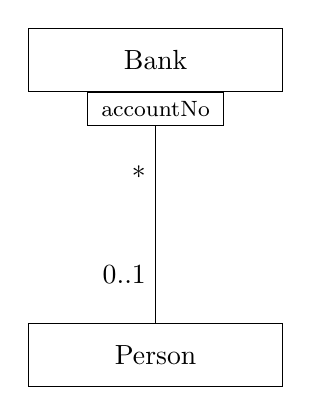
\begin{tikzpicture}
      \node [draw, rectangle, align=center, text width=3cm, minimum
      height=0.8cm] (A) {Bank} ;
      \node [draw, rectangle, align=center, text width=1.5cm, minimum
      height=0.3cm, below=0 of A] (Q) { \footnotesize accountNo } ;
      \node [draw, rectangle, align=center, text width=3cm, minimum
      height=0.8cm, below=2.5 of Q] (B) {Person} ;

      \path (Q.south) edge node [near start, left] {*} node [near end,
      left] {0..1} (B.north) ;
    \end{tikzpicture}

  }

  \only<3-4> {

  %\begin{center}
  %  \centering\includegraphics[width=0.8\hsize]{assoc-qualifier-case2-a.pdf}
  %\end{center}

  \centering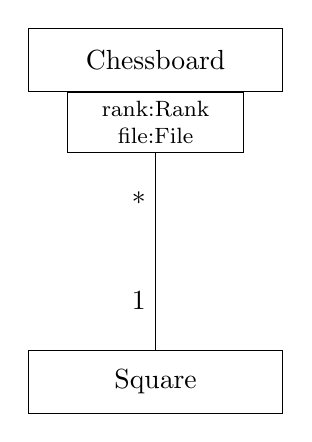
\begin{tikzpicture}
    \renewcommand\baselinestretch{0.8}
    \node [draw, rectangle, align=center, text width=3cm, minimum
    height=0.8cm] (A) {Chessboard} ;
    \node [draw, rectangle, align=center, text width=2cm, minimum
    height=0.3cm, below=0 of A] (Q) { \footnotesize rank:Rank \\ file:File } ;
    \node [draw, rectangle, align=center, text width=3cm, minimum
    height=0.8cm, below=2.5 of Q] (B) {Square} ;

    \path (Q.south) edge node [near start, left] {*} node [near end,
    left] {1} (B.north) ;
  \end{tikzpicture}
  }

  \only<5-6> {
  %\begin{center}
  %  \centering\includegraphics[width=0.7\hsize]{assoc-qualifier-case3-a.pdf}
  %\end{center}

  \centering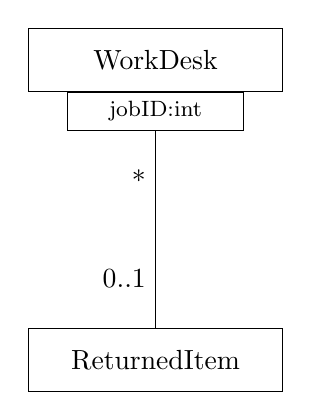
\begin{tikzpicture}
    \node [draw, rectangle, align=center, text width=3cm, minimum
    height=0.8cm] (A) {WorkDesk} ;
    \node [draw, rectangle, align=center, text width=2cm, minimum
    height=0.3cm, below=0 of A] (Q) { \footnotesize jobID:int} ;
    \node [draw, rectangle, align=center, text width=3cm, minimum
    height=0.8cm, below=2.5 of Q] (B) {ReturnedItem} ;

    \path (Q.south) edge node [near start, left] {*} node [near end,
    left] {0..1} (B.north) ;
  \end{tikzpicture}
  }

  \only<7-8> {
  %\begin{center}
    %\centering\includegraphics[width=0.7\hsize]{assoc-qualifier-case4-a.pdf}
  %\end{center}

    \centering\begin{tikzpicture}
    \node [draw, rectangle, align=center, text width=3cm, minimum
    height=0.8cm] (A) {订单} ;
    \node [draw, rectangle, align=center, text width=2cm, minimum
    height=0.3cm, below=0 of A] (Q) { \footnotesize 产品} ;

    \umlclass[y=-3.5, fill=white]{订单行}{amount:Number}{}
    \umlassoc[mult1=0..1]{订单行}{Q} 
    \end{tikzpicture}

  }
  \column{0.04\hsize}

  \only<2,4,6,8> {
    \centering{\Large \textcolor{red}{$\Rightarrow$} }
  }

  \column{0.48\hsize}

  \only<2> {
    %\begin{center}
    %\centering\includegraphics[width=0.6\hsize]{assoc-qualifier-case1-b.pdf}
    %\end{center}

    \centering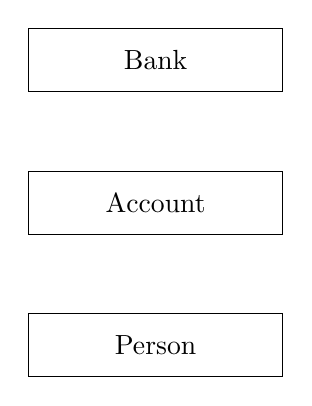
\begin{tikzpicture}
      \node [draw, rectangle, align=center, text width=3cm, minimum
      height=0.8cm] (A) {Bank} ;
      \node [draw, rectangle, align=center, text width=3cm, minimum
      height=0.8cm, below= of A] (Q) {Account } ;
      \node [draw, rectangle, align=center, text width=3cm, minimum
      height=0.8cm, below= of Q] (B) {Person} ;

      \umlassoc[mult1=1, mult2=*]{A}{Q}
      \umlassoc[mult1=1, mult2=*]{B}{Q}
    \end{tikzpicture}

  }

  \only<4> {
    %\begin{center}
    %\centering\includegraphics[width=0.8\hsize]{assoc-qualifier-case2-b.pdf}
    %\end{center}

    \centering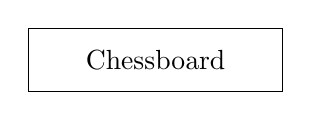
\begin{tikzpicture}
    \node [draw, rectangle, align=center, text width=3cm, minimum
    height=0.8cm] (A) {Chessboard} ;
    \umlclass[y=-3, fill=white] {Square}{ \footnotesize rank:Rank \\ file:File }{} ;
    \umlassoc[mult1=1, mult2=64]{A}{Square} ;
    \end{tikzpicture}

  }

  \only<6> {
    %\begin{center}
    %\centering\includegraphics[width=0.7\hsize]{assoc-qualifier-case3-b.pdf}
    %\end{center}

  \centering\begin{tikzpicture}
    \tikzumlset{fill class=white}
    \umlsimpleclass{WorkDesk} ;
    \umlsimpleclass[y=-2]{Job} ;
    \umlsimpleclass[y=-4]{ReturnedItem} ;
    \umlassoc[mult1=1, mult2=*]{WorkDesk}{Job}
    \umlassoc[mult1=1, mult2=*]{ReturnedItem}{Job}

  \end{tikzpicture}

  }

  \only<8> {
    %\begin{center}
    %\centering\includegraphics[width=0.65\hsize]{assoc-qualifier-case4-b.pdf}
    %\end{center}
    \centering\begin{tikzpicture}
    \node [draw, rectangle, align=center, text width=3cm, minimum
    height=0.8cm] (A) {订单} ;

    \umlclass[y=-2.5, fill=white]{订单行}{amount:Number}{}

    \node [draw, rectangle, align=center, text width=3cm, minimum
    height=0.8cm, below=of 订单行 ] (B) {产品} ;

    \umlaggreg[mult1=1, mult2=*]{A}{订单行} 
    \umlassoc[mult1=1, mult2=*]{B}{订单行} 
    \end{tikzpicture}


  }
  \end{columns}
  %\end{overlayarea}
\end{frame}

\begin{frame}
  \frametitle{UML2新增两种图形修饰}
    %\footnotesize
%\begin{tabular}{cc}
%\onslide<1->{\includegraphics[width=0.46\hsize]{assoc-qualifier-uml2-compos}} &
%\onslide<2->{\includegraphics[width=0.46\hsize]{assoc-qualifier-uml2-nav}}\\
%\onslide<1-> {聚合种类} & \onslide<2-> {可导航}\\
%& \\
%\onslide<3->{\includegraphics[width=0.46\hsize]{assoc-qualifier-uml2-notnav}} &
%\onslide<4->{\includegraphics[width=0.46\hsize]{assoc-qualifier-uml2-owner}}\\
%\onslide<3->{不可导航} & \onslide<4->{拥有权}\\
%& \\
%\onslide<5->{\includegraphics[width=0.46\hsize]{assoc-qualifier-uml2-many}}&
%\onslide<6->{\includegraphics[width=0.46\hsize]{assoc-qualifier-uml2-para}}\\
%\onslide<5->{多种修饰符同时使用} & \onslide<7->{悖论} \\
%\end{tabular}

  \footnotesize
  \begin{tikzpicture}
    \tikzumlset{fill class=white}
    \def\CW{3}
    \def\LX{3+\CW}
    \def\RX{\LX+\CW}

    \umlsimpleclass[width=1cm]{A}
    \umlsimpleclass[width=1cm, x=\CW]{B}
    \umlaggreg{A}{B}
    \node at (\CW/2, -0.5) {聚合种类} ;

    \umlsimpleclass[width=1cm, x=\LX]{A}
    \umlsimpleclass[width=1cm, x=\RX]{B}
    \umluniassoc{B}{A}
    \node at (\LX+\CW/2, -0.5) {可导航} ;

    \umlsimpleclass[width=1cm, y=-1.5]{A}
    \umlsimpleclass[width=1cm, x=\CW, y=-1.5]{B}
    \draw (B) -- node [cross out, draw, near end] {} (A) ;
    \node at (\CW/2, -2) {不可导航} ;

    \umlsimpleclass[width=1cm, x=\LX, y=-1.5]{A}
    \umlsimpleclass[width=1cm, x=\RX, y=-1.5]{B}
    \draw [-Circle] (B) -- node [near start, above]{endB} node [near
    end, above] {endA}  (A) ;
    \node at (\LX+\CW/2, -2) {拥有权} ;
    \node [below = 0 of B] {a:A[*]} ;
    \draw (B.south west) -- ++(0,-0.5) -| (B.south east) ;

    \umlsimpleclass[width=1cm, y=-3]{A}
    \umlsimpleclass[width=1cm, x=\CW, y=-3]{B}
    \draw [{Circle[] Straight Barb[width=6pt]}-{Rays [width=8pt] Diamond [open,
    width=6pt]}] (B) -- (A) ;
    \node at (\CW/2, -3.5) {多种修饰} ;

    \umlsimpleclass[width=1cm, x=\LX, y=-3]{A}
    \umlsimpleclass[width=1cm, x=\RX, y=-3]{B}
    \draw [-{Rays [width=8pt] Circle[] }] (B) -- node [near start, above]{endB} node [near
    end, above] {endA}  (A) ;
    \node [red] at (\LX+\CW/2, -3.5) {出现悖论} ;
  \end{tikzpicture}
\end{frame}

\begin{frame}[fragile]
  \frametitle{UML2新增了更多含在花括号内的特性串}
  \begin{tabular}{ll}
    \verb~{subsets <property-name>}~ &  子集合 \\
    \verb~{redefines <end-name>}~ &  重定义 \\
    \verb~{union}~  & 由它子集合的合并而派生 \\
    \verb~{ordered}~ &  有序集合 \\
    \verb~{nonunique}~ & 允许同一元素出现一次以上 \\
    \verb~{sequence}, {seq}~  & 序列 \\
  \end{tabular}
  \begin{alertblock}{注意UML2规范的定义说明}
    定义:(特性串)缺省表明关联端点代表了一个集合 \\
    解读:关联另一端的一个实例与本端的一组实例相关联
  \end{alertblock}
\end{frame}

\begin{frame}
  \frametitle{正确对待各种复杂概念}
  \begin{itemize}
    \item 不鼓励全面使用规范中定义的各种复杂概念
    \item 重点掌握基本概念,提高用基本概念解决问题的能力和技巧
    \item 尽可能用类、二元关联以及少数几种修饰建立清晰的模型
  \end{itemize}
  \vspace*{2ex}
  \pause
  \centering\Ovalbox{\hspace*{3cm} \Large \textbf{简单为美} \hspace*{3cm}}

\end{frame}

\subsection{如何建立关联}

\begin{frame}[t]
  \frametitle{如何建立关联}
  \begin{enumerate}
    \only<1>{
    \item 根据问题域和系统责任发现所需要的关联,
      哪些类的对象实例之间存在着对用户业务有意义的关系?
      \begin{itemize}
        \item 问题域中实际事物之间有哪些值得注意的关系?
        \item 这种信息是否需要通过有序对(或者$n$元组)来体现?
        \item 这些信息是否需要在系统中进行保存、管理或维护?
        \item 系统是否需要查阅和使用由这种关系所体现的信息?
      \end{itemize}
      \vspace*{1cm}
    \Ovalbox{\qquad 准则:关联确实为系统提供了\alert{\textbf{有用}}的信息 \qquad}
    }
    \only<2-4>{
    \setcounter{enumi}{1} 
    \item 简化复杂关联
      \begin{itemize}
        \item 对关联属性和操作的处理 
        \item 对n元关联的处理
        \item 避免一个类在关联中多次出现 
        \item 多对多关联的处理 
      \end{itemize}

    }

    \only<3> {
    %\begin{center}
    %\centering\includegraphics[width=0.7\hsize]{assoc-sup-cus-n2n.pdf}
    %\end{center}

      \vspace*{2ex}
      
      \centering\begin{tikzpicture}
        \tikzumlset{fill class=white}
        \umlemptyclass{供货商}
        \umlemptyclass[x=5]{客户}
        \umlassoc[mult1=*, mult2=*]{客户}{供货商}
      \end{tikzpicture}

    }
    \only<4> {

    %\begin{center}
    %\centering\includegraphics[width=0.7\hsize]{assoc-sup-cus-binary.pdf}
    %\end{center}
      \vspace*{2ex}
      \centering\begin{tikzpicture}
        \tikzumlset{fill class=white}
        \umlemptyclass{供货商}
        \umlemptyclass[x=5]{客户}
        \umlassoc[mult1=*, mult2=*]{客户}{供货商}
        \node [cross out, minimum width=0.6cm, draw=red, ultra thick] at (2.5, 0) {} ;
        \umlclass[x=2.5, y=-2]{供需合同}{卖方\\买方}{}
        \umlVHassoc[mult1=1, mult2=*, pos2=1.8]{供货商}{供需合同}
        \umlVHassoc[mult1=1, mult2=*, pos2=1.8]{客户}{供需合同}
      \end{tikzpicture}

    }
    \only<5>{
    \setcounter{enumi}{2} 
    \item 为关联端点添加修饰 
      \begin{itemize}
        \item 分析关联的多重性 
        \item 给出关联名或角色名
        \item 识别聚合种类
        \item 其他修饰
          \begin{itemize}
            \item 导航性、特性串等——根据实际情况决定是否采用
            \item 限定符——用简单的类和关联的概念解决
          \end{itemize}
      \end{itemize}
    \item 在类中设立实现关联的属性

    }
    \only<6> {
    \setcounter{enumi}{4} 
    \item 关联定位

      \vspace*{2ex}
    %\begin{center}
    %\centering\includegraphics[width=0.9\hsize]{assoc-locate.pdf}
    %\end{center}
      \centering\begin{tikzpicture}
        \tikzumlset{fill class=white}
        \umlemptyclass{计算机}
        \umlemptyclass[x=-4]{系统管理员}
        \umlemptyclass[x=-3, y=-4]{服务器}
        \umlemptyclass[y=-4]{客户机}
        \umlemptyclass[x=4, y=-4]{用户}
        \umlassoc[mult1=1, mult2=*]{系统管理员}{计算机}
        \umlassoc[mult1=*, mult2=1]{用户}{客户机}

        \umlinherit{客户机}{计算机}
        \umlVHVinherit{服务器}{计算机}

        \node at (2, -4.3) {使用} ;
        \node at (-1.8, 0.3) {操作} ;
      \end{tikzpicture}
    }
  \end{enumerate}
\end{frame}

\section{交互关系(消息)}

\subsection{概念与表示法}

\begin{frame}
  \frametitle{什么是消息}
  \only<1> {
  \begin{block}{现实生活中}
    人或其他事物之间传递的信息,例如:
    \begin{itemize}
      \item 人与人之间的对话、通信、发通知、留言 \\
      \item 交通信号灯对车辆和行人发出的信号 \\
      \item 人发给设备的遥控信号等 \ldots
    \end{itemize}
  \end{block}
}

  \only<2> {
  \begin{block}{软件系统中}
    进程或软件成分之间传送的信息
    \begin{itemize}
      \item \textcolor{blue}{控制信息}:  例如一次函数调用,或唤醒一个进程
      \item \textcolor{blue}{数据信息}:  例如传送一个数据文件
    \end{itemize}
  \end{block}
}

  \only<3> {
  \begin{block}{面向对象的系统中}
    (按严格封装的要求)消息是对象之间在行为上的唯一联系方式 
    \begin{itemize}
      \item 狭义: 消息是向对象发出的服务请求 
      \item 广义: 消息是对象之间在一次交互中所传送的信息
    \end{itemize}
  \end{block}

  \Ovalbox{ \quad 消息有发送者和接收者,遵守共同约定的语法和语义 \quad}
}
\end{frame}

\begin{frame}
  \frametitle{顺序系统中的消息}
  \begin{itemize}
    \item 每个消息都是向对象发出的服务请求, 最常见的是函数调用
    \item 消息都是同步的
    \item 接收者执行消息所请求的服务
    \item 发送者等待消息处理完毕再继续执行
    \item 每个消息只有唯一的接收者
  \end{itemize}
\end{frame}

\begin{frame}
  \frametitle{并发系统中的消息}
  \begin{block}{并发系统}
    是由多个任务并发执行的系统,系统中含有多个主动对象(或有一个主动对
    象,但它含有多个主动操作)和若干被动对象
  \end{block}
  \begin{block}{控制流}
    主动操作实现上对应并发执行的处理机调度单位\textcolor{blue}{进程}或
    \textcolor{blue}{线程},本书统称为控制流\\
    每个控制流是由一系列顺序执行的操作所构成的活动序列 \\
    控制流内部的消息和控制流之间的消息
  \end{block}
\end{frame}

\begin{frame}
  \frametitle{控制流间的消息}
  \begin{itemize}
      \only<1> {
    \item 消息的多种用途
      \begin{itemize}
        \item 服务请求
        \item 传送数据
        \item 发送通知
        \item 传递控制信号, \ldots
      \end{itemize}
      \begin{definition}
        消息是对象之间一次交互中所传送的信息
      \end{definition}
    }
    \only<2> {
    \item 消息的同步与异步
      \begin{block}{同步消息(synchronous)}
        仅当发送者要发送一个消息而且接收者已做好接收消息的准备时才能传送
        的消息
      \end{block}
      \begin{block}{异步消息(asynchronous)}
        发送者不管接收者是否做好接收准备都可以发送的消息
      \end{block}
      \begin{block}{限时消息(timeout)}
        当接收者未准备好时发送者只等待一个限定的时间
      \end{block}
    }
    \only<3> {
    \item 接收者对消息有不同响应方式
      \begin{itemize}
        \item 创建控制流响应消息
        \item 控制流已存在,立即响应
        \item 延迟响应
        \item 不响应
      \end{itemize}
    }
    \only<4> {
    \item 发送者对消息处理结果有不同期待方式
      \begin{itemize}
        \item 等待回应
        \item 事后查看结果
        \item 不等待不查看
      \end{itemize}
    }
    \only<5-> {
    \item 消息的接收者可能不唯一
      \begin{itemize}
        \item 定向消息(directed message)
        \item 广播消息(broadcast message)
      \end{itemize}
    }
  \end{itemize}
  \only<6> {
    \begin{alertblock}{OOA阶段不必考虑所有细节}
      并发系统消息的多样一方面来源于需求, 一方面来源于实现系统。OOA阶段
      应主要考虑需求问题
    \end{alertblock}
  }
\end{frame}

\begin{frame}
  \frametitle{消息对面向对象建模的意义}
  消息体现了对象之间的行为依赖关系,是实现对象之间的动态联系,使系统成为
  一个能运行的整体,并使各个部分能够协调工作的关键因素

  \begin{itemize}
    \item 在顺序系统中,消息体现了过程抽象的原则
    \item 在并发系统中
      \begin{itemize}
        \item 控制流内部的消息,使控制流内部呈现出清晰的脉络
        \item 控制流之间的消息,体现了控制流之间的通信关系
      \end{itemize}
  \end{itemize}
\end{frame}

\begin{frame}
  \frametitle{OO模型需要表示消息的哪些信息}
  重要性递降
    \begin{enumerate}
      \item 对象之间是否存在着某种消息?
      \item 这种消息是控制流内部的还是控制流之间的?
      \item 每一种消息是从发送者的哪个操作发出的?是由接收者的哪个操作响应
      和处理的?
    \item 消息是同步的还是异步的?
    \item 发送者是否等待消息的处理结果?
  \end{enumerate}
\end{frame}

\begin{frame}
  \frametitle{要不要在类图中表示消息}
  UML的处理方式: \\
  \quad 不在类图中表示消息,只在协作图和顺序图中表示 \\
  \quad 理由:把类图定义为静态结构图,不表示动态信息 \\
  \alert{问题}:\\
  \quad 类图中的``操作''本身就是动态信息 \\
  \quad 交互图是实例级的,抽象级别是个别实例 \\
  \quad 交互图的局部有限性
\end{frame}

\begin{frame}
  \frametitle{各种箭头}
  \begin{tabular}{llp{5cm}}
    箭头种类 & 图形符号 & 用途 \\ \hline
  实线开放箭头 & \tikz{\draw[thick, ->,>=angle 90] (0,0) -- (2,0);} & 关
  联的导航性(类图), 异步消息(顺序图) \\
  虚线开放箭头 & \tikz{\draw[dotted, thick, ->,>=angle 90] (0,0) --
  (2,0);} & 依赖(类图、包图、用况图、构件图), 
  从消息接收者的操作返回(顺序图)\\
  实线封闭箭头 & \tikz{\draw[thick, ->,>=triangle 45] (0,0) -- (2,0);} &
  同步消息(顺序图、协作图)\\
\end{tabular}
\end{frame}

\begin{frame}
  \frametitle{借用依赖关系表示类图中的消息}
  控制流内部消息:\\
  \qquad \tikz{\draw[dotted, very thick, ->,>=angle 90] (0,0) -- node[above,
  pos=0.8] {$\scriptstyle «call» $} (4,0);}

  \vspace*{1cm}
  控制流之间消息:\\
  \qquad \tikz{\draw[dotted, very thick, ->,>=angle 90] (0,0) -- node[above,
  pos=0.8] {$\scriptstyle «send» $} (4,0);}

\end{frame}

\begin{frame}
  \frametitle{表示法示例}
  \only<1> {
    %\begin{center}
    %\centering\includegraphics[width=1.0\hsize]{msg-notation-case1.pdf}
    %\end{center}
    \begin{tikzpicture}
      \tikzumlset{fill class=white}
      \umlemptyclass{C}
      \umlemptyclass[y=-4]{D}
      \umlemptyclass[x=-4, type=active]{A}
      \umlemptyclass[x=4]{E}
      \umlemptyclass[x=-4, y=-4, type=active]{B}
      \umlemptyclass[x=4, y=-4]{F}
      \umldep[stereo=call]{A}{C}
      \umldep[stereo=call]{C}{E}
      \umldep[stereo=call]{B}{D}
      \umldep[stereo=call]{D}{F}
      \umldep[stereo=call]{E}{F}
      \umldep[stereo=send]{D}{C}
    \end{tikzpicture}
  }
  \only<2> {
    %\begin{center}
    %\centering\includegraphics[width=0.75\hsize]{msg-notation-case2.pdf}
    %\end{center}

    \begin{tikzpicture}
      \tikzumlset{fill class=white}
      \umlemptyclass[type=active, x=-3] {生产者}
      \umlemptyclass[type=active, x=3] {消费者}
      \umlclass[y=-2]{缓冲区}{}{存数据\\取数据 \\挂起\\唤醒}
      \umlVHdep[stereo=call]{生产者}{缓冲区}
      \umlVHdep[stereo=call]{消费者}{缓冲区}
      \umldep[recursive=-30|-90|2cm, stereo=send]{缓冲区}{缓冲区}
    \end{tikzpicture}
  }
\end{frame}

\subsection{如何建立消息}

\begin{frame}
  \frametitle{建立控制流内部的消息}
  \Ovalbox{\qquad \qquad 策略——“操作模拟”和“执行路线追踪” \qquad \qquad}
  \begin{enumerate}
    \item 模拟当前对象操作的执行,考虑需要其它对象提供什么服务
    \item 判断该消息是否属于同一个控制流:   
      \begin{itemize}
        \item 二者应该顺序地执行还是并发地执行?   
        \item 是否引起控制流的切换?   
        \item 接收者是否只有通过当前消息的触发才能执行?
      \end{itemize}
      \item 向接收者画出消息连接线,填写模型规约,重复上述工作到当前操作模拟完毕
      \item 对控制流内部的每一种消息,重复上述工作
      \item 针对每个主动类的每个主动操作重复上述工作,检查疏漏
    \end{enumerate}
\end{frame}

\begin{frame}
  \frametitle{建立控制流之间的消息}
  对每个控制流考虑以下问题:
  \begin{enumerate}
    \item 执行时是否需要请求其他控制流中的对象提供服务?
    \item 执行时是否要和其他控制流中的对象交互数据?
    \item 执行时是否将产生某些可影响其他控制流执行的事件?
    \item 各控制流之间是否需要相互传递一些同步控制信号?
    \item 一个控制流将在何种条件下中止执行?在它中止之后将在何种条件下被唤
  醒?由哪个控制流唤醒?
  \end{enumerate}

  从上述各个角度发现控制流之间的消息,在相应的类之间画出消息连接线 

\end{frame}

\section{依赖关系}

\subsection{依赖关系}

\begin{frame}
  \frametitle{什么是依赖(dependency)}
  \textcolor{blue}{UML1.4对依赖的定义和解释}
  \begin{quote}
  “依赖:两个建模元素之间的一种关系,其中一个建模元素(独立元素)的一个
  改变将影响到另一个建模元素(依赖元素)。”
\end{quote}

\textcolor{blue}{Booch等《UML用户指南》的解释}
   \begin{quote}
   “两个事物之间的语义关系,其中一个事物(独立事物)的改变将影响到另一个
   事物(依赖事物)。”
 \end{quote}

\end{frame}

\begin{frame}
  \frametitle{UML2对依赖关系的新阐述}
  \begin{quote}
     “依赖表明模型元素之间的供方/客方(supplier /client)关系,其中供方
     的修改可能影响到客方元素。依赖意味着,如果没有供方,客方的语义就是
     不完整的。依赖在一个模型中出现并不含有任何运行时的语义,它完全是以
     参与这种关系的模型元素的名义而不是以其实例的名义给出的。”
   \end{quote}

   \alert{\textbf{认识}:} \\
   \begin{itemize}
     \item 依赖着眼于表达纸面上的模型元素之间的关系,而不是这些元素所描述的
       客观事物在问题域中的固有关系
     \item 依赖基本上不能视为一种面向对象的概念
   \end{itemize}
\end{frame}

\begin{frame}
  \frametitle{依赖的多种情况: UML1}
    %\begin{center}
    %\centering\includegraphics[width=1.0\hsize]{dep-uml1.pdf}
    %\end{center}
  \centering\begin{tikzpicture}
    \tikzumlset{fill class=white}
    \umlsimpleclass{Dependency}
    \umlsimpleclass[x=-4, y=-2]{Abstraction}
    \umlsimpleclass[x=-1.5, y=-2, width=1cm]{Usage}
    \umlsimpleclass[x=1.5, y=-2, width=1cm]{Permission}
    \umlsimpleclass[x=4, y=-2, width=1cm]{Binding}
    \umlVHVinherit{Abstraction}{Dependency}
    \umlVHVinherit{Usage}{Dependency}
    \umlVHVinherit{Permission}{Dependency}
    \umlVHVinherit{Binding}{Dependency}

    \renewcommand\baselinestretch{1.0}
    \node [dashed, rectangle callout, draw, callout absolute
    pointer={(Abstraction.south)}, text width=1.5cm, align=left] at (-3,
    -4) {<<derive>> \\ <<refine>> \\ <<realize>> \\ <<trace>>} ;
    \node [dashed, rectangle callout, draw, callout absolute
    pointer={(Usage.south)}, text width=2.5cm, align=left] at (0,
    -4.2) {<<call>> \\ <<create>> \\ <<instantiate>> \\ <<responsibility>>
    \\ <<send>>} ;
    \node [dashed, rectangle callout, draw, callout absolute
    pointer={(Permission.south)}, text width=2cm, align=left] at (3.1,
    -3.7) {<<access>> \\ <<friend>> \\ <<import>>} ;
  \end{tikzpicture}
\end{frame}

\begin{frame}
  \frametitle{依赖的多种情况: UML2}
    %\begin{center}
    %\centering\includegraphics[width=1.0\hsize]{dep-uml2.pdf}
    %\end{center}
  \centering\begin{tikzpicture}
    \tikzumlset{fill class=white}
    \umlsimpleclass{Dependency}
    \umlsimpleclass[x=-2, y=-2]{Abstraction}
    \umlsimpleclass[x=1.5, y=-2]{Usage}
    \umlsimpleclass[x=-2, y=-3.5]{Realization}
    \umlsimpleclass[x=-2, y=-5]{Substitution}
    \umlVHVinherit{Abstraction}{Dependency}
    \umlVHVinherit{Usage}{Dependency}
    \umlinherit{Realization}{Abstraction}
    \umlinherit{Substitution}{Realization}

    \renewcommand\baselinestretch{1.0}
    \node [dashed, rectangle callout, draw, callout absolute
    pointer={(Abstraction.west)}, text width=1.5cm, align=left] at (-4.7,
    -3) {<<derive>> \\ <<refine>> \\ <<trace>>} ;
    \node [dashed, rectangle callout, draw, callout absolute
    pointer={(Usage.east)}, text width=2.5cm, align=left] at (4.3,
    -3.5) {<<call>> \\ <<create>> \\ <<instantiate>> \\ <<responsibility>>
    \\ <<send>>} ;
  \end{tikzpicture}
\end{frame}

\begin{frame}[t, label=current]
  \frametitle{其他外观类似的表示}
    %\begin{center}
    %\centering\includegraphics[width=0.9\hsize]{dep-notation.pdf}
    %\end{center}

    \tikz \draw [thick, dashed, -Straight Barb] (0, 0) -- node [near
    end, above] {<<关键词>>} (4, 0) ;

  \only<1> {

    \begin{enumerate}
      \item 作为依赖关系标准衍型的关键词
    \end{enumerate}

    \renewcommand\baselinestretch{1.0}

    \tikz \node [align=left] {<<instantiate>> \\
      <<create>> \\
      <<call>> \\
      <<derive>> \\
      <<refine>> \\
      <<responsibility>> \\
      <<send>> \\
    <<trace>> };

    
  }
  \only<2> {
    \begin{enumerate}
      \setcounter{enumi}{1} 
      \item 用于依赖但未明确称为标准衍型的关键词
    \end{enumerate}

    \tikz \node [align=left] {<<abstraction>> \\
      <<realize>> \\
      <<substitute>> \\
      <<permit>> \\
      <<use>> } ;
  }
  \only<3> {
    \begin{enumerate}
      \setcounter{enumi}{2} 
      \item 附加于虚线开放箭头但不称为依赖关系的关键词
    \end{enumerate}

    \tikz \node [align=left] {<<access>> \\
      <<apply>> \\
      <<bind>> \\
      <<extend>> \\
      <<import>> \\
      <<include>> \\
      <<manifest>> \\
      <<occurrence>> \\
      <<represents>> } ;
  }
 
\end{frame}

\begin{frame}
  \frametitle{依赖关系对面向对象建模的作用}
  \begin{itemize}
    \item 继承、聚合、关联、消息这四种关系中都已经蕴涵了依赖的含义,不需
      要再用依赖关系再做重复的表示

    \item 除了上述关系之外,在OO建模中没有多少重要的信息必须用依赖关系表达
    \item 由于UML没有在类图中提供消息的表示法,可以借用依赖关系来表示类
      图中的消息
  \end{itemize}
  \begin{alertblock}{注意}
    避免建立语义含糊不清的依赖关系,更要避免用这些含糊不清的依赖关系代替
    含义明确的OO关系
  \end{alertblock}
\end{frame}

\end{document}
